\documentclass[border = 15pt, multi, tikz]{standalone}

\usepackage{import}
\usepackage{fontspec}

% \setmainfont{Times New Roman}
% \setsansfont{Times New Roman}

\subimport{./layers/}{init}

\usetikzlibrary{positioning}
\usetikzlibrary{3d}
\usetikzlibrary{fit}
\usetikzlibrary{backgrounds}
\usetikzlibrary{calc}

\def\ConvColor{rgb: yellow, 5; red, 2.5; white, 5}
\def\ConvReluColor{rgb: yellow, 5; red, 5; white, 5}
\def\PoolColor{rgb: red, 1; black, 0.3}
\def\NormColor{rgb: green, 3; blue, 2; white, 7}
\def\FcColor{rgb: blue, 5; red, 2.5; white, 5}
\def\FcReluColor{rgb: blue, 5; red, 5; white, 4}
\def\SoftmaxColor{rgb: pink, 5; black, 0}
\definecolor{LineGrey}{HTML}{6A6A6A}
\definecolor{cEEGb}{RGB}{232, 142, 58}
\def\skipRed{rgb: red, 9; white, 1}



\begin{document}

\begin{tikzpicture}
    \tikzstyle{connection} = [
        ultra thick,
        every node/.style={sloped, allow upside down},
        draw = \edgecolor,
        opacity = 0.72
    ]
    \tikzstyle{branch} = [
        very thick,
        draw = \edgecolor,
        opacity = 0.72,
        -{Stealth[length = 4mm, width = 2.6mm]}
    ]
    \tikzstyle{skip} = [
        line width = 1.5pt,
        draw = \skipRed,
        opacity = 0.65,
        densely dashed,
        -{Stealth[length = 3mm, width = 2mm]}
    ]

    \node[anchor = west, font = \bfseries\Large] at (6.25, 6.15) {MTNet — Multimodal Transformer Architecture};
    \node[anchor = west, font = \large\itshape, text = LineGrey] at (4, 5.2) {EEG and eye-tracking streams are encoded separately, then fused in a 128-node hidden layer};

    \node[anchor = east, font = \bfseries\large, text = cEEGb] at (-1.72, 5.2) {EEG branch};

    \node[canvas is zy plane at x = -1, inner sep = 0pt] (eegimage) at (-2.85, 1.55, 0) {
        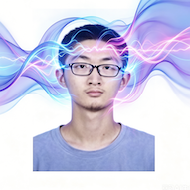
\includegraphics[width = 5cm, height = 5cm]{./demo.png}
    };

    \coordinate (eegimageout) at (-3, 1.55, 0);

    \pic[shift = {(-1.45, 1.55, 0)}] {
        RightBandedBox = {
            name = eeg,
            caption = \mbox{EEG input},
            xlabel = {{"20", "9"}},
            zlabel = ,
            fill = \ConvColor,
            bandfill = \ConvReluColor,
            height = 28,
            width = {3.2, 3.2},
            depth = 24,
            scale = 0.17
        }
    };

    \node[anchor = west, font = \normalsize, rotate = 45] at ($(eeg-east) + (-0.75, -3.5)$) {64 channels};

    \draw [connection] (eegimageout) -- node {\midarrow} (eeg-west);

    \pic[shift = {(1.55, 0, 0)}] at (eeg-east) {
        RightBandedBox = {
            name = band,
            caption = Band split,
            xlabel = {{"9", ""}},
            zlabel = ,
            fill = \ConvColor,
            bandfill = \ConvReluColor,
            height = 26,
            width = {3.2, 3.2},
            depth = 22,
            scale = 0.17
        }
    };

    \node[anchor = west, font = \normalsize, rotate = 45] at ($(eeg-east) + (1.9, -3.25)$) {$4\textrm{Hz}\sim40\textrm{Hz}$};

    \pic[shift = {(1.50, 0, 0)}] at (band-east) {
        RightBandedBox = {
            name = spatial,
            caption = Spatial filter,
            xlabel = {{"", "288"}},
            zlabel = ,
            fill = \ConvColor,
            bandfill = \ConvReluColor,
            height = 23,
            width = {2.5, 2.5},
            depth = 20,
            scale = 0.17
        }
    };

    \node[anchor = west, font = \normalsize, rotate = 45] at ($(eeg-east) + (4.5, -2.75)$) {channels};

    \pic[shift = {(1.50, 0, 0)}] at (spatial-east) {
        RightBandedBox = {
            name = temporal,
            caption = Temporal conv,
            xlabel = {{"40", ""}},
            zlabel = ,
            fill = \ConvColor,
            bandfill = \ConvReluColor,
            height = 20,
            width = {3.0, 3.0},
            depth = 18,
            scale = 0.17
        }
    };

    \node[anchor = west, font = \normalsize, rotate = 45] at ($(eeg-east) + (6.75, -2.75)$) {kernels};

    \pic[shift = {(1.5, 0, 0)}] at (temporal-east) {
        Box = {
            name = bnelu,
            caption = ,
            xlabel = {{"\textbf{BN} + \textbf{ELU}", ""}},
            fill = \NormColor,
            opacity = 0.72,
            height = 11,
            width = 1.8,
            depth = 13,
            scale = 0.17
        }
    };

    \pic[shift = {(2.75, 0, 0)}] at (temporal-east) {
        Box = {
            name = pool,
            caption = \hspace*{-1.25em}\vspace*{2em}\mbox{Avg pool},
            xlabel = {{"", ""}},
            fill = \PoolColor,
            opacity = 0.55,
            height = 14,
            width = 1.0,
            depth = 14,
            scale = 0.17
        }
    };

    \pic[shift = {(1.75, 0, 0)}] at (pool-east) {
        RightBandedBox = {
            name = tokens,
            caption = Tokens,
            xlabel = {{"12", "40"}},
            zlabel = ,
            fill = \FcColor,
            bandfill = \FcReluColor,
            height = 4,
            width = {3.2, 3.2},
            depth = 42,
            scale = 0.17
        }
    };

    \pic[shift = {(1.85, 0, 0)}] at (tokens-east) {
        RightBandedBox = {
            name = qkv,
            caption = QKV,
            xlabel = {{"Q", "K", "V"}},
            zlabel = ,
            fill = \FcColor,
            bandfill = \FcReluColor,
            height = 4,
            width = {4, 4, 4},
            depth = 42,
            scale = 0.17
        }
    };

    \pic[shift = {(1.55, 0, 0)}] at (qkv-east) {
        RightBandedBox = {
            name = mhsa,
            caption = MHSA,
            xlabel = {{"8", "heads"}},
            zlabel = ,
            fill = \FcColor,
            bandfill = \FcReluColor,
            height = 4,
            width = {3.2, 3.2},
            depth = 42,
            scale = 0.17
        }
    };

    \pic[shift = {(1, 0, 0)}] at (mhsa-east) {
        Box = {
            name = normone,
            caption = Add \& Norm,
            xlabel = {{"", ""}},
            fill = \NormColor,
            opacity = 0.72,
            height = 4,
            width = 2.2,
            depth = 42,
            scale = 0.17
        }
    };

    \pic[shift = {(2.25, 0, 0)}] at (mhsa-east) {
        RightBandedBox = {
            name = ffn,
            caption = FFN,
            xlabel = {{"", ""}},
            zlabel = ,
            fill = \FcColor,
            bandfill = \FcReluColor,
            height = 4,
            width = {3.1, 3.1},
            depth = 42,
            scale = 0.17
        }
    };

    \pic[shift = {(1, 0, 0)}] at (ffn-east) {
        Box = {
            name = normtwo,
            caption = Add \& Norm,
            xlabel = {{"", ""}},
            fill = \NormColor,
            opacity = 0.72,
            height = 4,
            width = 2.2,
            depth = 42,
            scale = 0.17
        }
    };

    \begin{scope}[on background layer]
        \node [
            draw = LineGrey,
            densely dashed,
            line width = 1.5pt,
            rounded corners = 5pt,
            inner xsep = 5pt,
            inner ysep = 50pt,
            fit = (qkv-northwest)(qkv-nearsouthwest)(normtwo-northeast)(normtwo-nearsoutheast),
            label = {[font = \bfseries\large, fill = white, inner sep = 2pt]above = 18pt: Transformer encoder ($N=4,\ h=8$)}
        ] (transformerbox) {};
    \end{scope}

    \draw [skip] (qkv-north) .. controls +(0, 1) and +(0, 2) .. (normone-north);
    \draw [skip] (normone-north) .. controls +(0, 1) and +(0, 2) .. (normtwo-north);

    \pic[shift = {(3.25, 0, 0)}] at (ffn-east) {
        RightBandedBox = {
            name = fusion,
            caption = Fusion,
            xlabel = {{"128", ""}},
            zlabel = ,
            fill = \FcColor,
            bandfill = \FcReluColor,
            height = 5,
            width = {3.0, 3.0},
            depth = 44,
            scale = 0.17
        }
    };

    \node[anchor = west, font = \normalsize, rotate = 45] at ($(eeg-east) + (26, -2.25)$) {hidden};

    \pic[shift = {(1.5, 0, 0)}] at (fusion-east) {
        Box = {
            name = softmax,
            caption = \mbox{MD / HC},
            xlabel = {{"2", ""}},
            zlabel = ,
            fill = \SoftmaxColor,
            opacity = 0.82,
            height = 4,
            width = 4,
            depth = 4,
            scale = 0.17
        }
    };

    \draw [connection] (eeg-east) -- node {\midarrow} (band-west);
    \draw [connection] (band-east) -- node {\midarrow} (spatial-west);
    \draw [connection] (spatial-east) -- node {\midarrow} (temporal-west);
    \draw [connection] (temporal-east) -- node {\midarrow} (pool-west);
    \draw [connection] (pool-east) -- node {\midarrow} (tokens-west);
    \draw [connection] (tokens-east) -- node {\midarrow} (qkv-west);
    \draw [connection] (qkv-east) -- node {\midarrow} (mhsa-west);
    \draw [connection] (mhsa-east) -- node {\midarrow} (ffn-west);
    \draw [connection] (ffn-east) -- node {\midarrow} (fusion-west);
    \draw [connection] (fusion-east) -- node {\midarrow} (softmax-west);

    \node[anchor = west, font = \bfseries\large, text = cEEGb] at (2, -5) {Eye-tracking branch};

    \pic[shift = {(8.45, -3.80, 0)}] {
        RightBandedBox = {
            name = etfeat,
            caption = AOI,
            xlabel = {{"3", ""}},
            zlabel = ,
            fill = \FcColor,
            bandfill = \FcReluColor,
            height = 4,
            width = {2.6, 2.6},
            depth = 28,
            scale = 0.17
        }
    };

    \pic[shift = {(1.55, 0, 0)}] at (etfeat-east) {
        RightBandedBox = {
            name = etvec,
            caption = 60-d vector,
            xlabel = {{"60", ""}},
            zlabel = ,
            fill = \FcColor,
            bandfill = \FcReluColor,
            height = 4,
            width = {2.5, 2.5},
            depth = 28,
            scale = 0.17
        }
    };

    \pic[shift = {(1.55, 0, 0)}] at (etvec-east) {
        RightBandedBox = {
            name = etfc,
            caption = FC expand,
            xlabel = {{"540", "1"}},
            zlabel = ,
            fill = \FcColor,
            bandfill = \FcReluColor,
            height = 4,
            width = {3.5, 3.5},
            depth = 28,
            scale = 0.17
        }
    };

    \draw [connection] (etfeat-east) -- node {\midarrow} (etvec-west);
    \draw [connection] (etvec-east) -- node {\midarrow} (etfc-west);

    \coordinate (etfcToFusion) at (etfc-west -| fusion-south);
    \draw [branch] (etfc-west) -- (etfcToFusion) -- (fusion-south);
\end{tikzpicture}

\end{document}